\section{Energy scale calibration}

\subsection{Resolution Scans}
\label{sec:resolution_scans}
As the signal from the detector is rather weak, the detector is connected to an
amplifying circuit as described in Section~\ref{sec:calibration:set-up}. However
there is a trade-off associated with this procedure as amplification also
applies to noise in the detector. In order to increase the signal strength the
voltage applied to the detector can be increased which in turn increases the
amount of signal electrons and leads to a stronger output signal. Along with
this comes though an increased probability for spontaneous discharges along
impurities and dirt remaining in the detector despite extensive cleaning
procedures as described in Section~\ref{sec:construction}.

As the two possibilities for varying the output signal strength are associated
with independent increases of noise and accordingly reduction of resolution we
are performing resolution scans for the two samples we are interested in
measuring: Americium and iron.

In order to reliably determine the resolution a Gaussian is fitted to the sample
peak previously identified in the multi-channel analyser (MCA) spectrum. We look
at the variable peak width divided by the peak position in order to determine
the resolution of our peak. For the peak width we are using the full-width
half-maximum (FWHM) value. As secondary decays will affect especially the lower
end of a the decay Gaussian \todo{how are they called exactly? secondary seems
  wrong} shape we are defining regions of interest (ROI) in which the Gaussian
is fitted.

The spectra obtained for americium (figure \ref{fig:scan:americium}) and iron
(figure \ref{fig:scan:iron}) are presented in appendix~\ref{app:resolution-scans} for different gains and voltages.
A gaussian is fitted to the marked ROI (blue lines) and the obtained channel number as well as
full-width half-maximum (FWHM) in channels are denoted in the figure.

The obtained parameters from the fit are plotted in figures
\ref{fig:resolution:americium} and \ref{fig:resolution:iron} for americium and
iron respectively. The uncertainties are propagated from the fit. Additional the
total uncertainty on the FWHM contains a \SI{10}{\percent} systematic
uncertainty due to the dependency on choosing the corresponding ROI.

\begin{figure}[htb]
  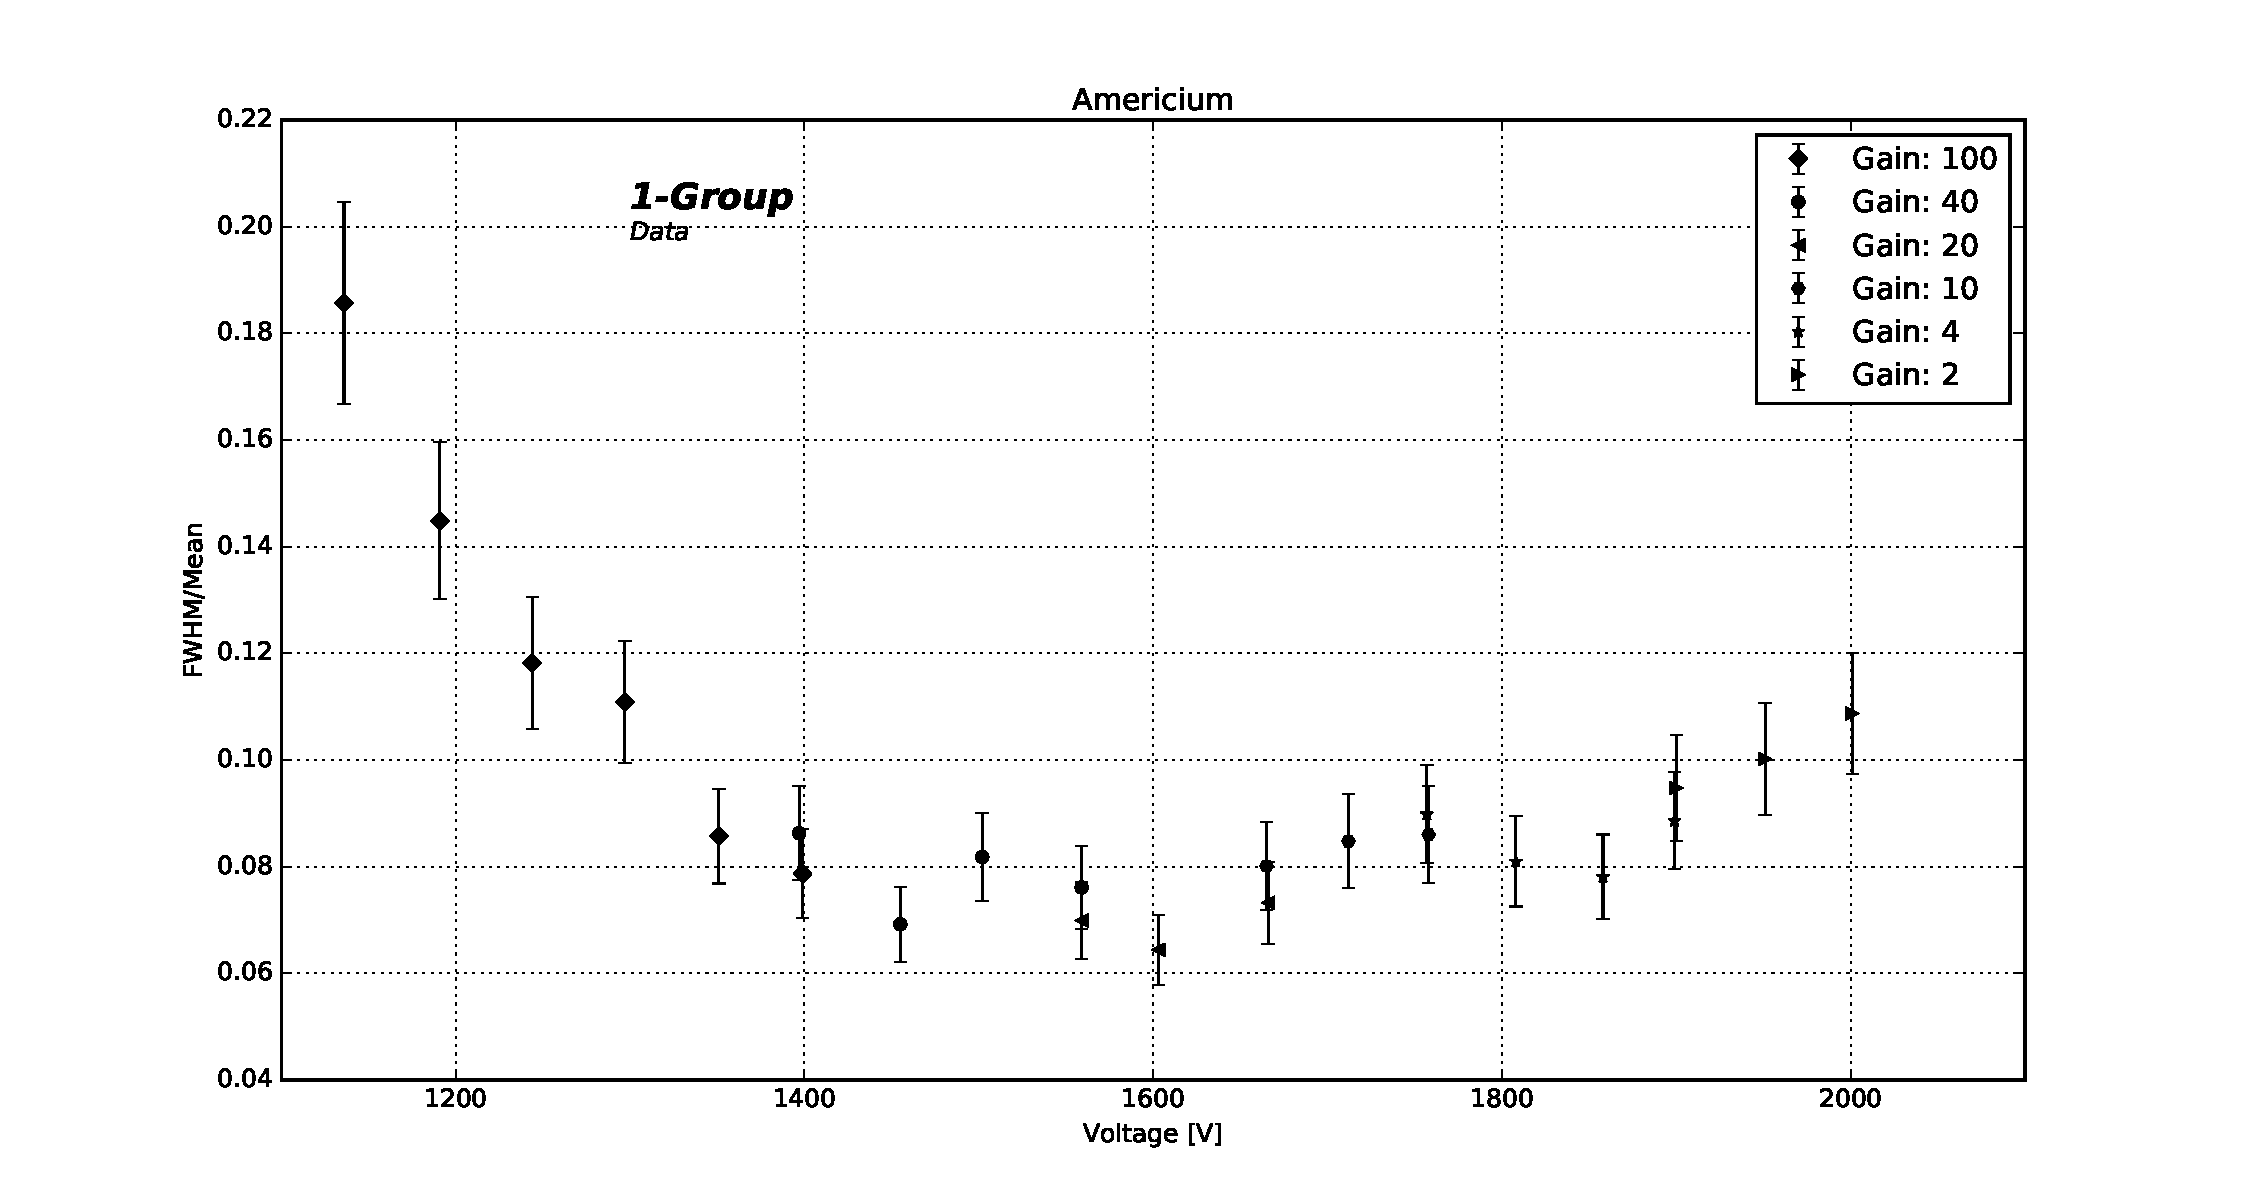
\includegraphics[width=\linewidth]{graphics/americium_scan}
  \caption{Americium scan}
  \label{fig:resolution:americium}
\end{figure}

\begin{figure}[htb]
  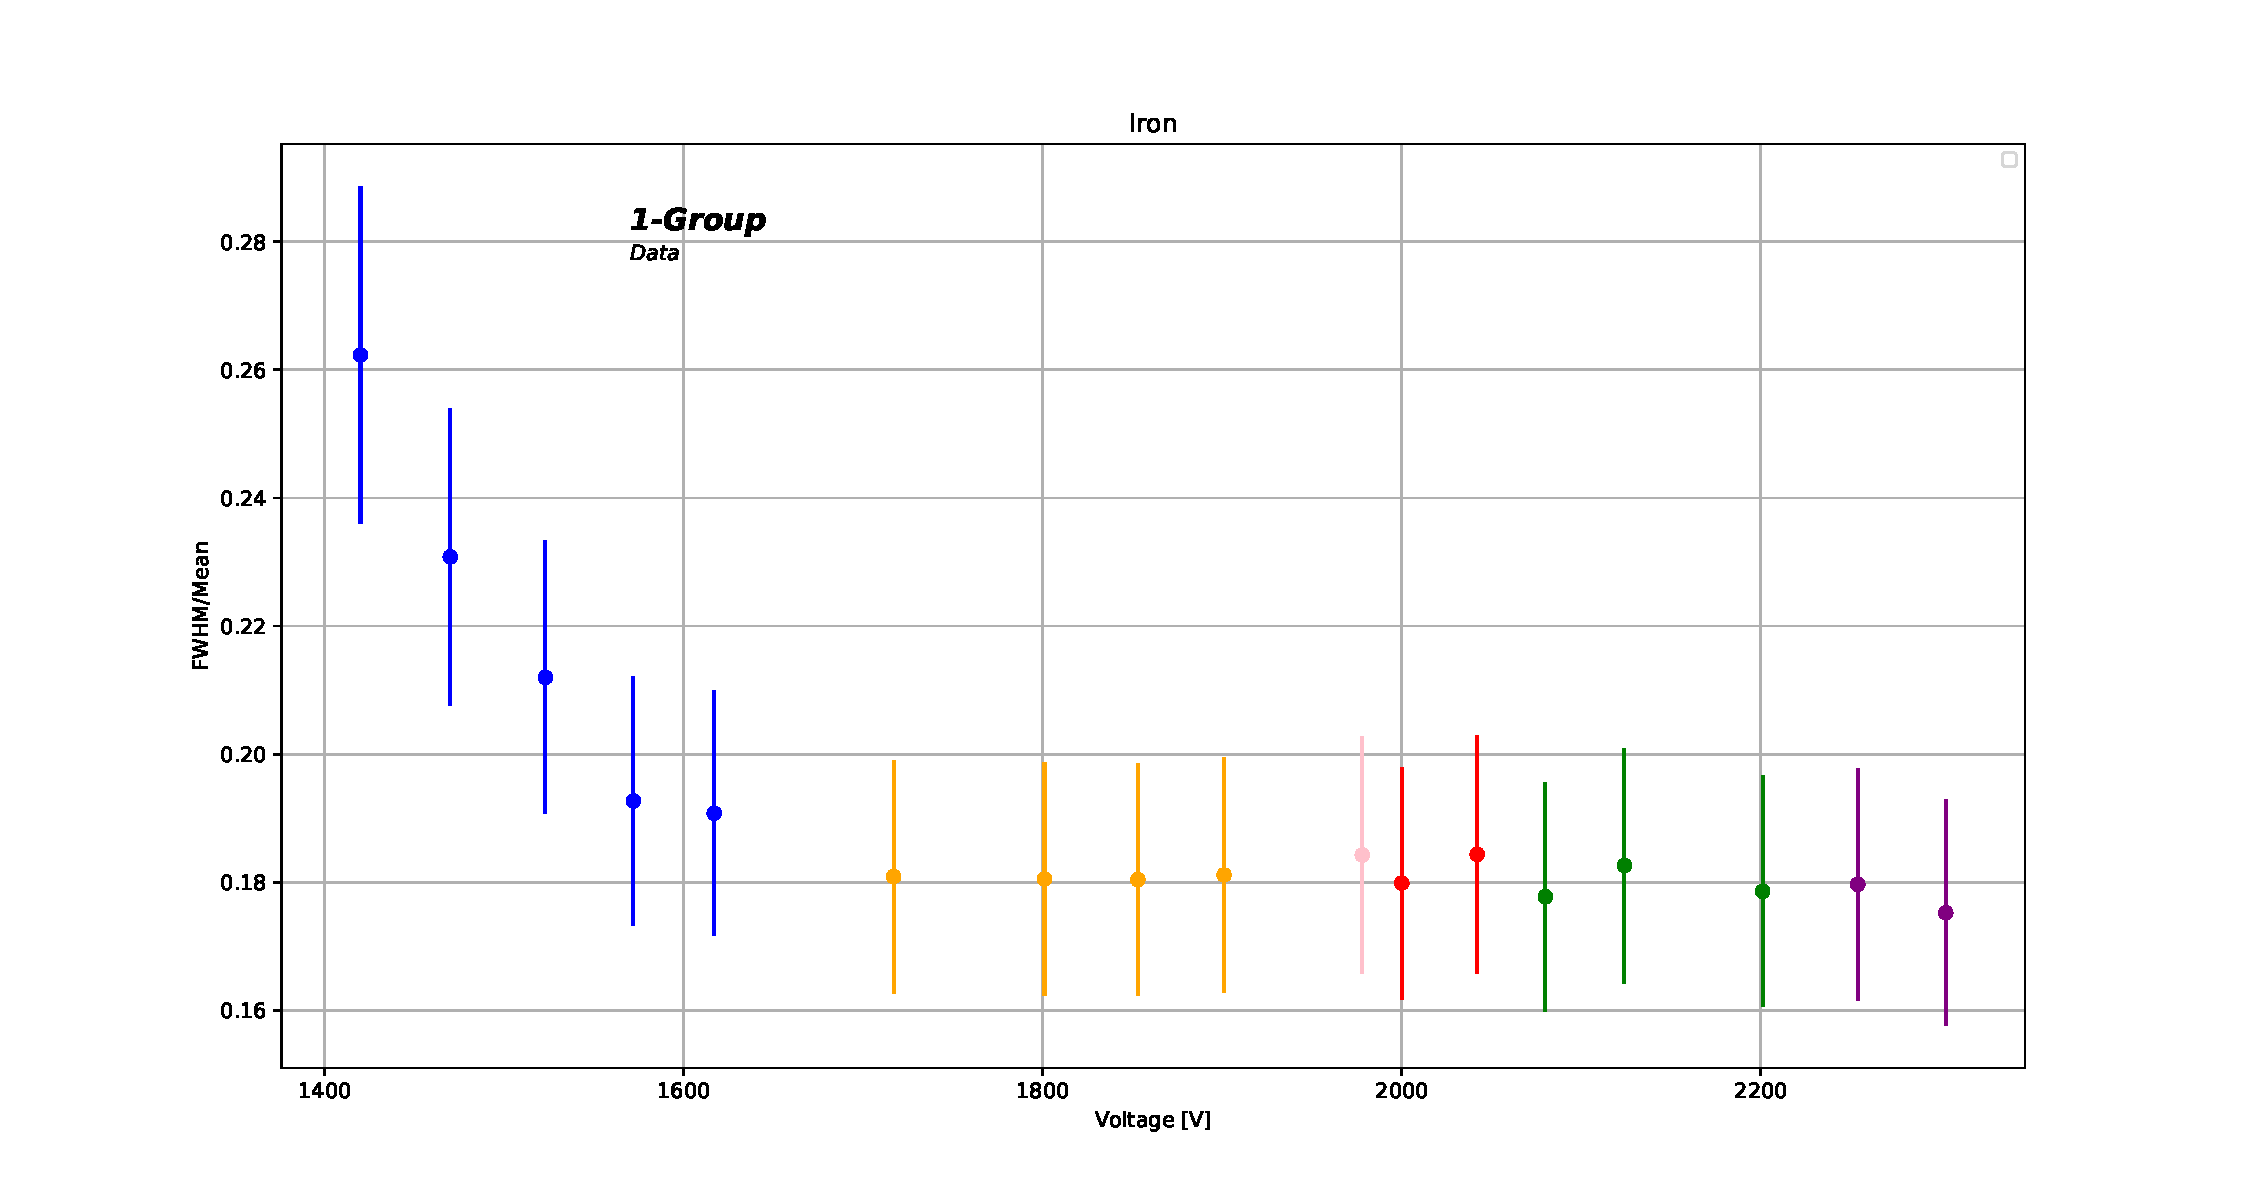
\includegraphics[width=\linewidth]{graphics/iron_scan}
  \caption{Iron scan}
  \label{fig:resolution:iron}
\end{figure}
